\section{Relaciones entre sitios de taxis, choferes y taxis}

A continuación se analizan las tres representaciones propuestas para las
relaciones entre sitios de taxis, choferes y taxis.

\begin{figure}[htbp]
  \centering
  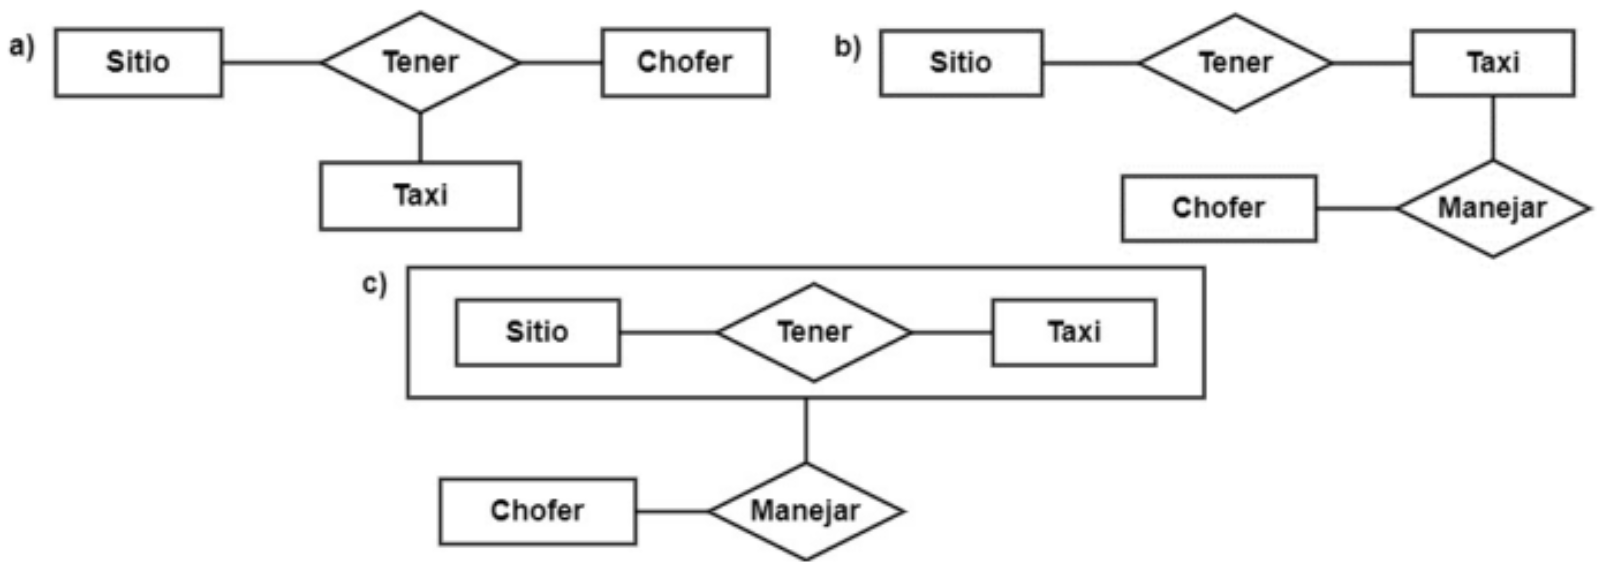
\includegraphics[width=0.94\textwidth]{../Diagramas/Ejercicio 2i.png}
  \caption{Representaciones propuestas en el ejercicio 2-i.}
  \label{fig:sitios-taxis}
\end{figure}

\begin{itemize}
    \item Indica qué diagramas representan la información requerida por las siguientes solicitudes de información:
          ¿Qué taxis maneja el chofer Raúl López en el sitio Santa Fe?, ¿A qué sitios está afiliado el chofer Carlos Reyes?,
          ¿Qué taxis están asociados al sitio Universidad?

        Los diagramas a) y c) conservan de forma explícita la asociación
        conjunta entre sitio, chofer y taxi. Por ello permiten contestar las
        tres consultas sin combinar hechos independientes. En b), las
        relaciones binarias indican qué taxis tiene un sitio y cuáles maneja
        un chofer, pero no garantizan que la combinación obtenida corresponda
        a una asignación real de ese chofer en ese sitio.

    \item ¿Qué modificación harías en el diagrama de la figura a), sin perder información, para que se puedan conocer qué
          taxis que maneja cada chofer?
        
        Se agrega una relación binaria \textbf{Maneja} entre \textbf{Chofer}
        y \textbf{Taxi}, sin eliminar la relación ternaria. La nueva relación
        registra los taxis que puede manejar cada chofer con independencia
        del sitio, mientras \textbf{Tener} conserva la asignación concreta de
        los tres participantes. Debe imponerse además que toda asignación
        ternaria proyecte un par presente en \textbf{Maneja}.

    \item ¿Qué diferencia existe entre los diagramas de las figuras a) y c)?
    
        El diagrama a) representa un único hecho ternario: una instancia sólo
        tiene significado por la combinación de los tres participantes. El
        diagrama c) primero forma el hecho \textbf{Tener} entre sitio y taxi y
        después lo trata como una unidad agregada que participa en
        \textbf{Manejar}. La agregación hace explícito que el chofer maneja un
        taxi en cuanto éste se encuentra asociado con un sitio.

    \item Cómo modificarías el diagrama de la figura a) para representar las siguientes restricciones:
          Un chofer no puede manejar más de un taxi en el mismo sitio. Un taxi no puede ser manejado por más de un chofer en el mismo sitio.

        En la relación ternaria se establecen dos restricciones de llave. La
        combinación $(\textit{Sitio},\textit{Chofer})$ determina a lo sumo un
        \textit{Taxi}; simétricamente,
        $(\textit{Sitio},\textit{Taxi})$ determina a lo sumo un
        \textit{Chofer}. En notación con flechas, se dirige una flecha hacia
        \textbf{Taxi} y otra hacia \textbf{Chofer}. No se dirige una flecha
        hacia \textbf{Sitio}, porque el mismo par chofer--taxi podría aparecer
        en sitios distintos si las reglas del dominio lo permiten.

\end{itemize}
